% !TEX root = ../main.tex
\subsection{Constraints on Galaxy Pitch angle}
Our hierarchical model identifies the pitch angle of individual arms ($\phi_\mathrm{arm}$) with less than {1.6\degree} of uncertainty for 95\% of arms, assuming no error on disc inclination and position angle. The pitch angle of a galaxy as a whole ($\phi_\mathrm{gal}$), however, is not well constrained. This is primarily a result of only having pitch angles measurements for a small number of arms per galaxy, and reflects the difficulty in providing a single value for the pitch angle of a galaxy containing individual arms with very different pitch angles. For galaxies with two arms identified in \textit{Galaxy Builder}, we have a mean uncertainty of ($\sigma_{\phi_\mathrm{gal}}$) of  {7.8\degree}, which decreases to {6.7\degree} and {5.8\degree} for galaxies with three and four arms respectively. This is consistent with the standard error on the mean for a galaxy with $N$ arms,

\begin{equation}
  \sigma_{\phi_\mathrm{gal}} = \frac{\sigma_\mathrm{gal}}{\sqrt{N}},
\end{equation}

where $\sigma_\mathrm{gal}$ is our measure of inter-arm variability of pitch angle and has a posterior distribution of $11.0^\circ\pm 1.0^\circ$. This variability is similar to the finding of \citet{2014ApJ...790...87D} and emphaises the need for fitting algorithms to not assume all arms have the same pitch angle.

\subsection{Dependence of pitch angle on Galaxy Morphology}
\label{section:morphology_comparision}
In order to test the possible progenitor distribution of our estimated arm pitch angles, we repeatedly perform an Anderson-Darling test \citep{10.2307/2286009} over each draw present in the MC trace, resulting in a distribution of Anderson-Darling statistics. We will refer to this test as the \textit{marginalized Anderson-Darling test}. We also make use of the two-sample Anderson-Darling \citep{doi:10.1080/01621459.1987.10478517} and Kolmogorov-Smirnov tests in a similar manner for comparison.

\subsubsection{Pitch angle vs. Bulge size}
We define a bulge prominence from Galaxy Zoo 2 as Equation 3 in \citet{2019MNRAS.487.1808M}:

\begin{equation}
  B_\mathrm{avg} = 0.2p_\mathrm{just noticeable} + 0.8p_\mathrm{obvious} + 1.0p_\mathrm{dominant}.
\end{equation}

We see no correlation between galaxy pitch angle derived from the hierarchical model and $B_\mathrm{avg}$. The Pearson correlation coefficient between the expectation value of galaxy pitch angle ($E(\phi_\mathrm{gal})$) and $B_\mathrm{avg}$ is -0.09. We see a slight correlation between $E(\phi_\mathrm{gal})$ and the fraction of volunteers who said a galaxy did not have a bulge (Pearson correlation coefficient of 0.19).

\comment{Do we need to do an Anderson-Darling test here?}

We separate our sample into ``weaker bulged galaxies'' and ``stronger bulged galaxies'' using , in order to examine whether they could be drawn from significantly different distributions. A marginalized two-sample Anderson-Darling test does not find any evidence that the samples were drawn from different distributions; we do not reject the null hypothesis at the 1\% level for any samples. The distribution of Anderson-Darling test statistics is shown in the upper panel of Figure \ref{fig:ad-morphology-test}.


\subsubsection{Pitch angle vs. Bar Strength}
We see no correlation between galaxy pitch angle derived from the \textit{hierarchical normal model} and Galaxy Zoo 2's debiased \textit{pbar}, which is widely viewed as a good measure of bar strength, and therefore a measure of the torque applied on the disc gas.

Separating the sample based off of $\mathrm{\textit{pbar}} > 0.5$, and restricting to galaxies with more than 10 classifications for \textit{pbar} (as performed by \citealt{2011MNRAS.411.2026M} and \citealt{2017MNRAS.469.3363K}) and performing a marginalized two-sample Anderson-Darling test does not find that the samples were drawn from different distributions (we reject the null hypothesis at the 1\% level for only 1\% of samples). The distribution of Anderson-Darling test statistics is shown in the lower panel of Figure \ref{fig:ad-morphology-test}.

We do not account for variation in bulge size in this work, however predictions from Manifold theory should not be affected as bulges do not provide a non-axisymmetric focing.

\begin{figure*}
  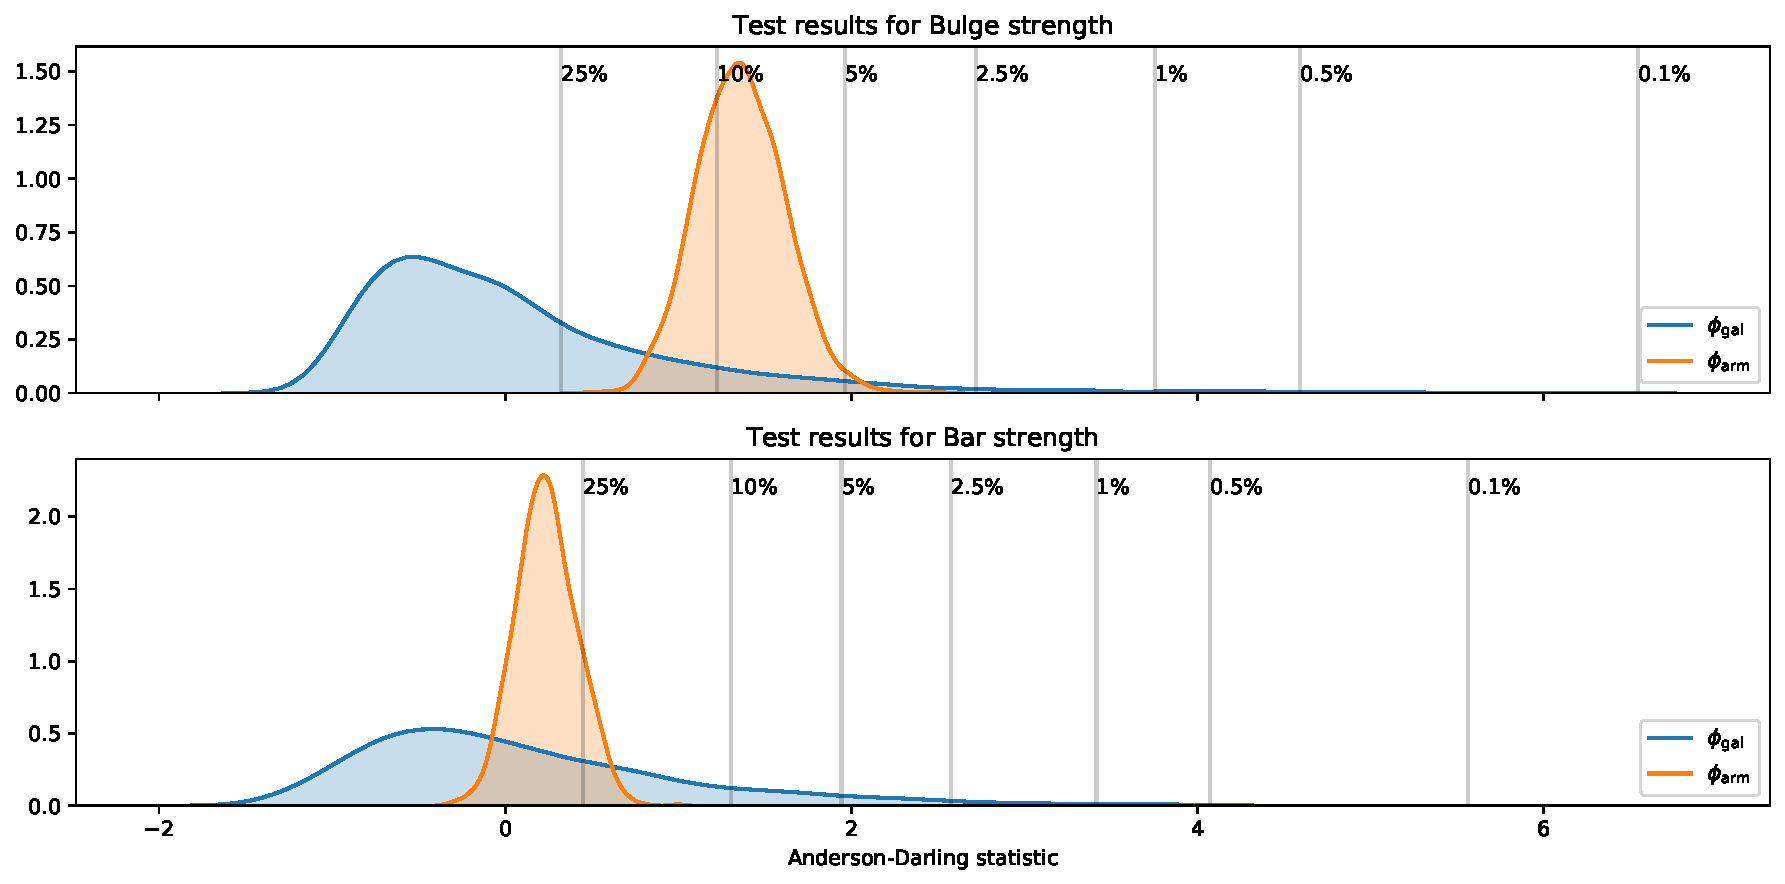
\includegraphics[width=17.7cm]{plots/bulge_bar_test_results.pdf}
  \caption{The results of marginalized two-sample Anderson-Darling tests examining whether pitch angles for Bulge-dominated and Disc-dominated galaxies are drawn from the same distribution (top panel), and the results of the same test for strongly-barred vs unbarred galaxies (bottom panel).}
  \label{fig:ad-morphology-test}
\end{figure*}


\subsection{Spiral Winding}
\label{section:spiral_winding}

For transient and reccurent spiral arms driven by self-gravity, \citet{2019arXiv190910291P} suggest that spiral patterns form at some maximum pitch angle ($\phi_\mathrm{max}$), continually wind up over time and finally dissapate at some minimum pitch angle ($\phi_\mathrm{min}$). They propose that, under a set of very simple assumptions, the evolution of pitch angle would be governed by

\begin{equation}
  \label{eq:winding}
  \cot{\phi} = \left[R\frac{\mathrm{d}\Omega_p}{\mathrm{d}R}\right](t - t_0) + \cot{\phi_\mathrm{max}},
\end{equation}

where $\Omega_p$ is the radially dependant pattern speed of the spiral arm and $t_0$ is the initial time at which it formed.

In QSDW theory, the pattern speed $\Omega_p$ is a constant in R, as spiral arms obey rigid-body rotation. If $\Omega_p$ instead varies with radius we would expect $\cot{\phi}$ to be uniformly distributed between $\cot{\phi_\mathrm{max}}$ and $\cot{\phi_\mathrm{min}}$.

In order to test this theory, \citet{2019arXiv190910291P} used a Kolmogorov-Smirnov test to examine the consistency of a sample of observed galaxy pitch angles with one uniform in cot. Pitch angles were measured using discrete fourier transformations in one- and two-dimensions, and as such do not account for inter-arm variations. They chose limits of $\cot{\phi} \in [1.00, 4.75]$ (roughly $11.9^\circ < \phi < 45.0^\circ$), motivated by examination of their data.

We aim to replicate their work here, using our sample and methods. We will make use of the marginalized tests described above, and examine winding on a per-arm basis, as well as a per-galaxy basis. Observation of the distribution of arm pitch angles in our sample suggests limits of $15^\circ < \phi < 50.0^\circ$.

\subsubsection{Galaxy Pitch angle}

Testing the uniformity in cot of $\phi_\mathrm{gal}$, between the limits specified above, using a marginalized Anderson-Darling test, results in rejecting the null hypothesis at the 1\% level for 68\% of samples. This suggests that a cot uniform model is not a good fit to galaxy pitch angle, but is not conclusive enough for us to unilaterally reject winding governed by Equation \ref{eq:winding}. The full distribution of Anderson-Darling statistics can be seen in the upper panel of Figure \ref{fig:ad-cot-test}.

This inconclusive result is perhaps unsurprising; were we to assume that spiral arms are transient and reccurent instabilities, there is little reason for all of the arms to be at precisely the same evolutionary stage at the same time. This is supported by the large spread in inter-arm pitch angles.


\subsubsection{Arm Pitch angle}
If we assume that spirals form and wind independantly in a galaxy and that their evolution over time can be described by Equation \ref{eq:winding}, the distribution of pitch angles of individual arms should be uniform in cot between our limits.

Using the marginalized Anderson-Darling test we cannot reject the null hypothesis at the 10\% level for any of the possible realizations of arm pitch angle. The resulting distribution of Anderson-Darling statistics in the lower panel of Figure \ref{fig:ad-cot-test}. This result is highly consistent with the model for spiral winding proposed by \citet{2019arXiv190910291P}, and can be seen as evidence that spirals are formed through local disc perturbations, and are primarily governed by local forces.

\begin{figure*}
  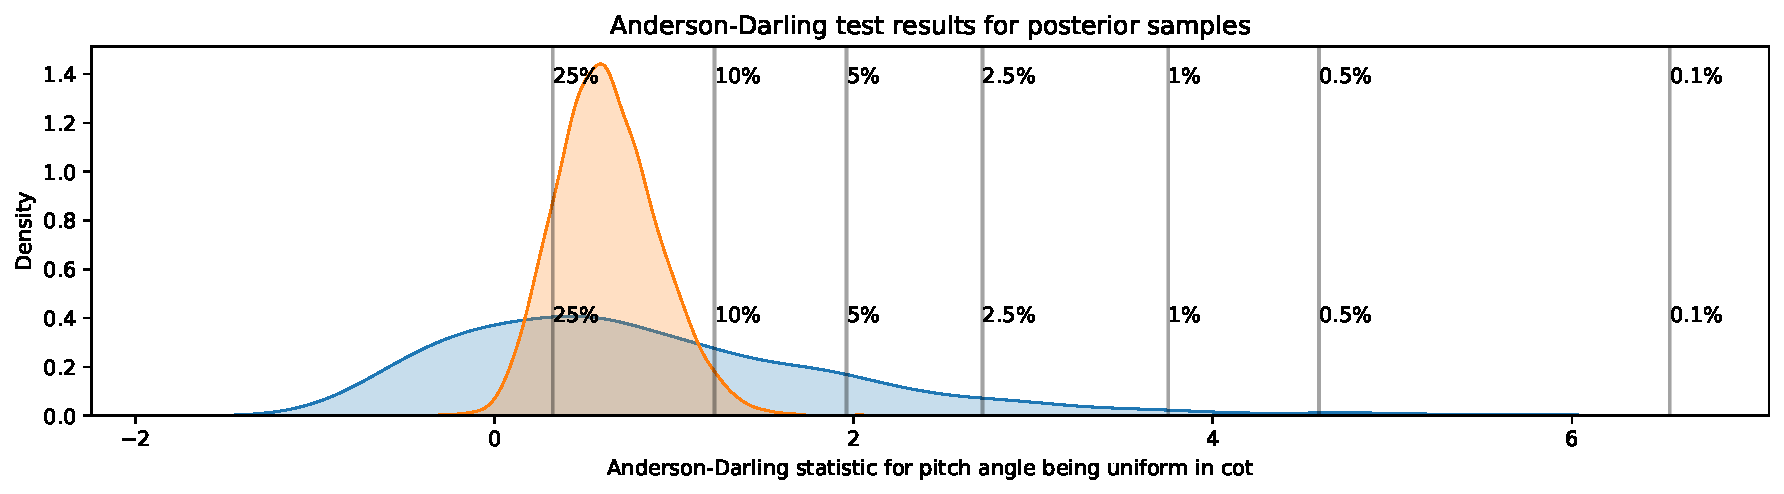
\includegraphics[width=17.7cm]{plots/combined_cot_uniform_marginalized_tests.pdf}
  \caption{The results of a marginalized Anderson-Darling test for uniformity in $\cot$ for $\phi_\mathrm{gal}$ (top panel) and $\phi_\mathrm{arm}$ (bottom panel), with values corresponding to various confidence intervals shown. Moving rightwards on the x-axis implies greater confidence in rejecting the null hypothesis.}
  \label{fig:ad-cot-test}
\end{figure*}


This result is highly sensitive to the lower limit of $\phi_\mathrm{gal}$ chosen; decreasing it to 10\degree results in us rejecting the cot-uniform progenitor at greater than the 0.1\% level for every realization of the posterior. As we have no information available on the biases present in \textit{Galaxy Builder} spiral arm classification, we should use the higher limits.

\comment{We do not account for observation effects, instead assuming that galaxy builder spiral arms are equally likely to be identified and recovered at all pitch angles. We also assume that the galaxy builder is representative of the general spiral population, which is not necessarily the case}
